\section{Results}

\subsection{Model calibration}

\begin{figure}
  \centering
  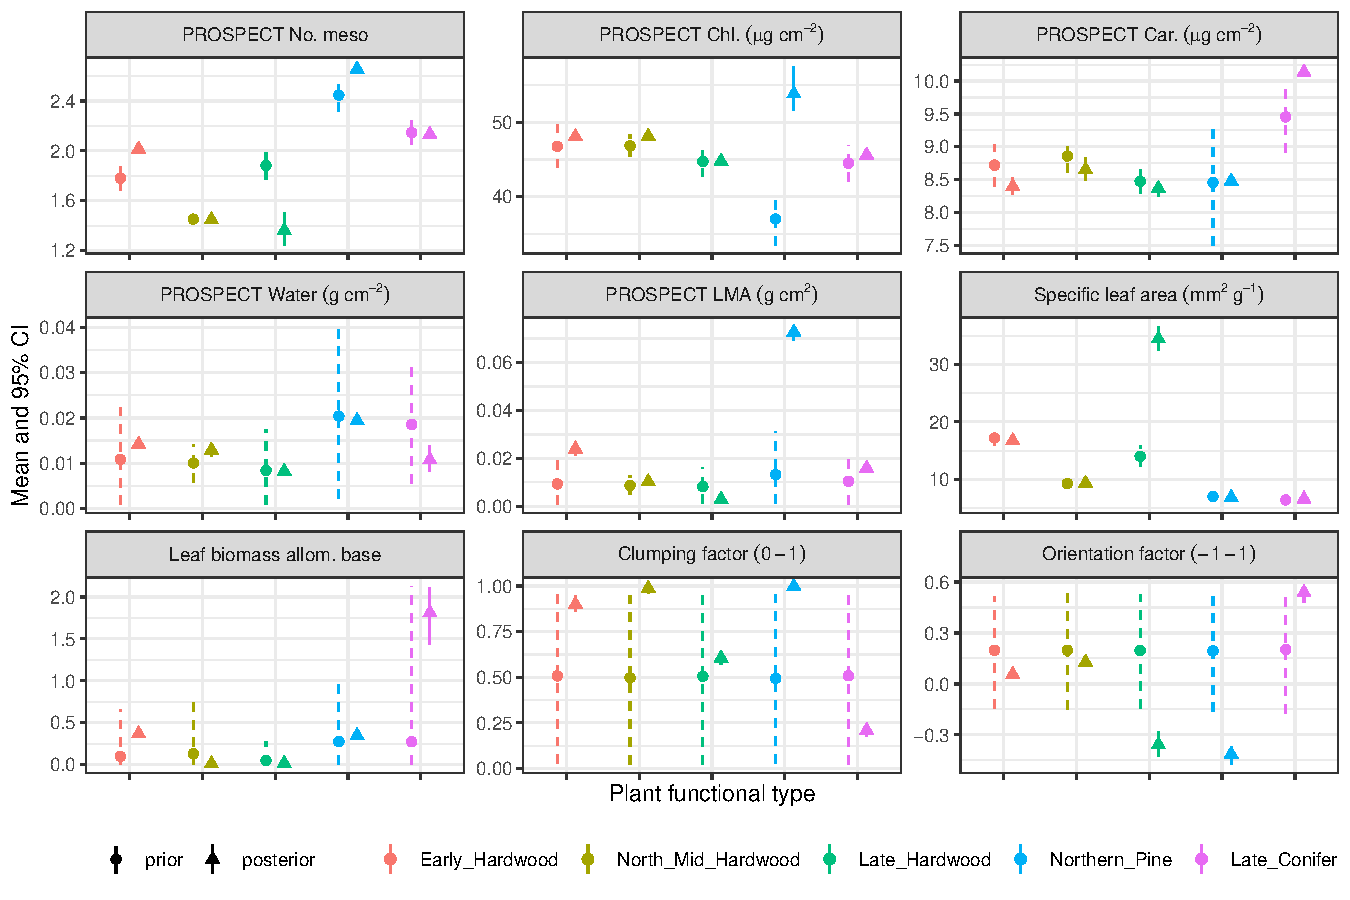
\includegraphics[width=\textwidth]{4_edr/figures/explore_spectra/pda_summary.pdf}
  \caption{\
    Summary statistics for model calibration parameter prior and posterior distributions.
  }\label{fig:pda_posteriors}
\end{figure}

Model calibration substantially improved the precision of almost all parameter estimates, even when prior distributions were strongly informative (Figure~\ref{fig:pda_posteriors}).
In most cases, the posterior distribution fell within the prior, but there were a few notable exceptions.
Specifically, northern pines had significantly higher calibration estimates of chlorophyll content and leaf mass per area and significantly lower estimates of the orientation factor (though the prior on the latter was not based on data).
Late hardwoods also had orientation factor estimates much lower than the prior, and also had significantly lower estimates of leaf mesophyll structure.

\begin{figure}
  \centering
  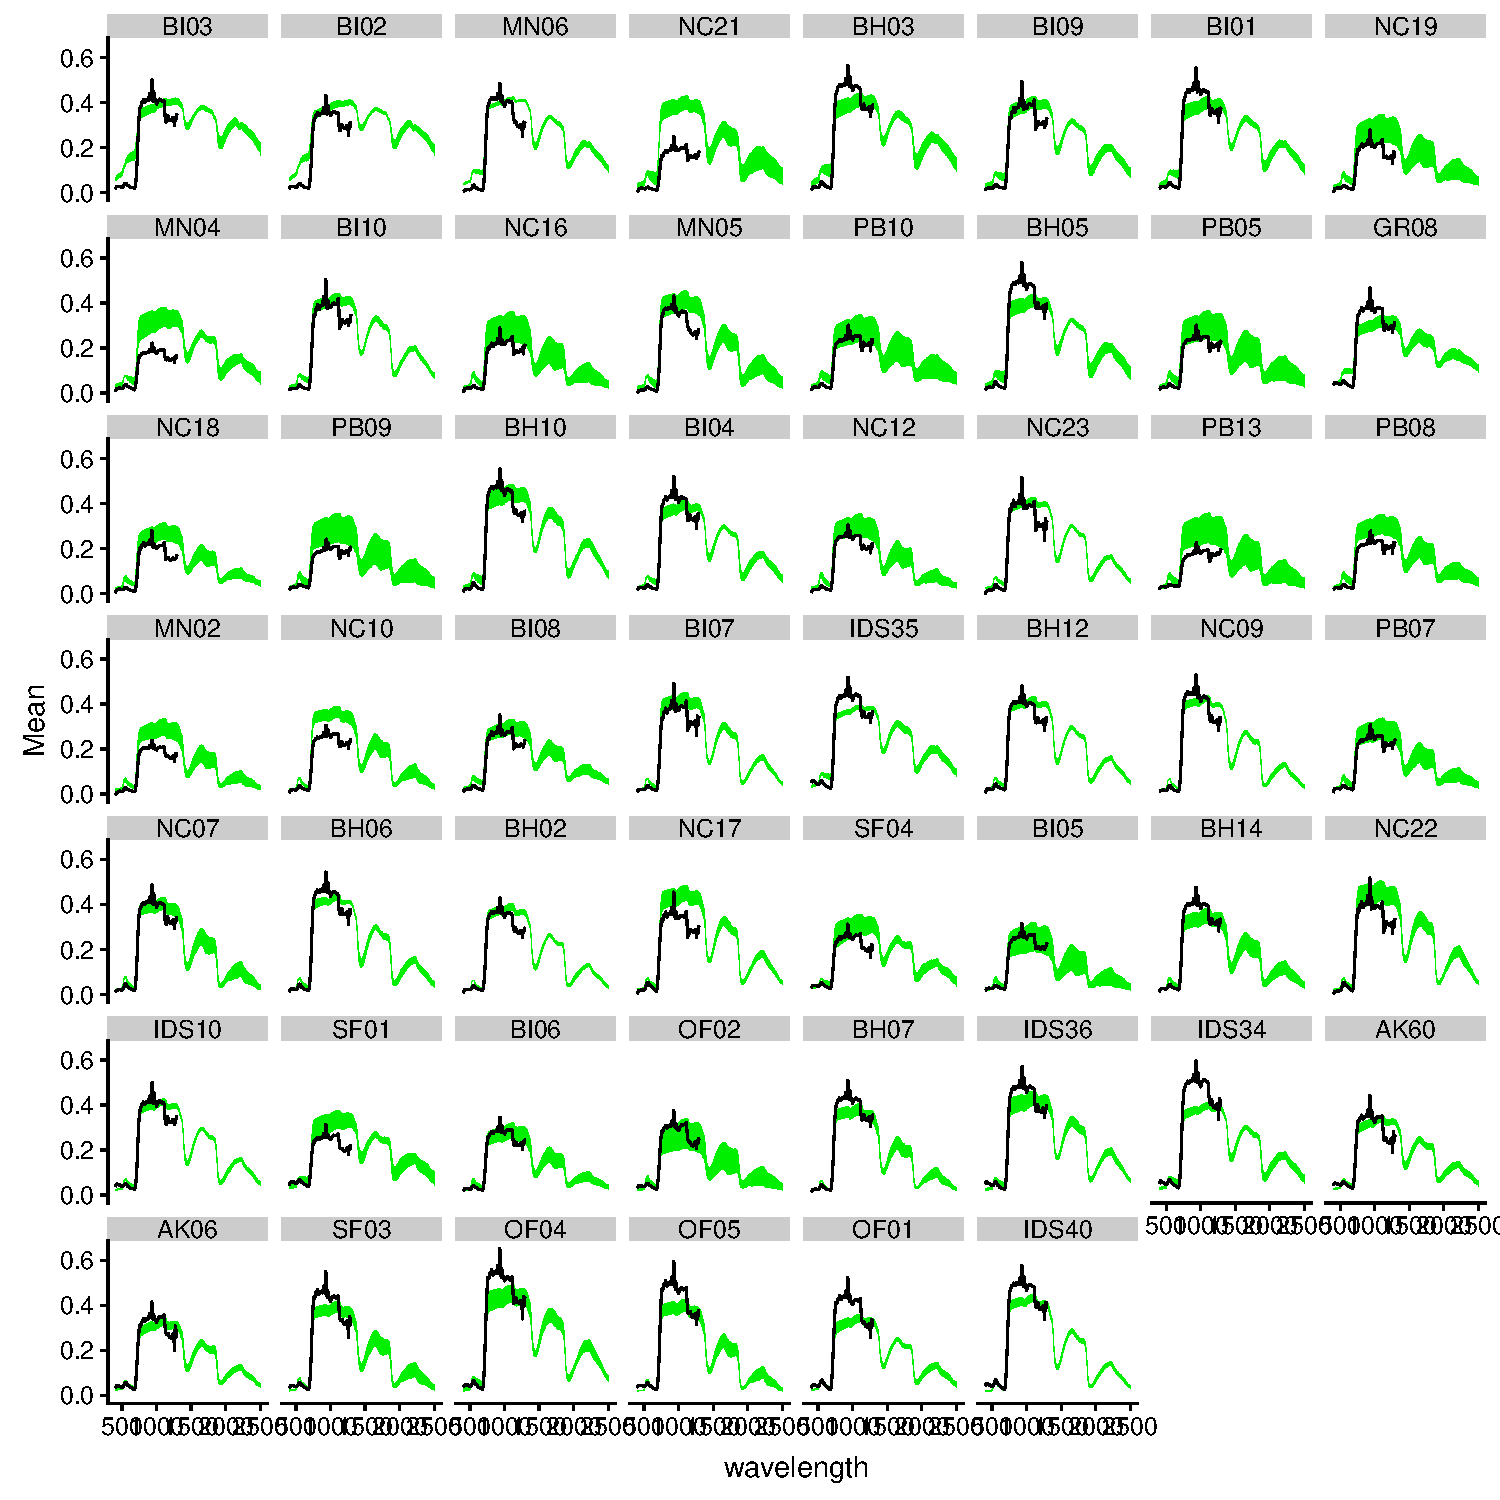
\includegraphics[width=\textwidth]{4_edr/figures/explore_spectra/errors_byvis_all.pdf}
  \caption{%
    Comparison between AVIRIS observations and posterior credible intervals on EDR predicted spectra for each site used in the calibration.
    Sites are sorted in order of decreasing mean bias in the visible ($<$750 nm) spectral region.
  }\label{fig:spec_error_all}
  % TODO: Put the CI on top, and make it transparent
  % TODO: Rotate x axis labels
\end{figure}

\begin{figure}
  \centering
  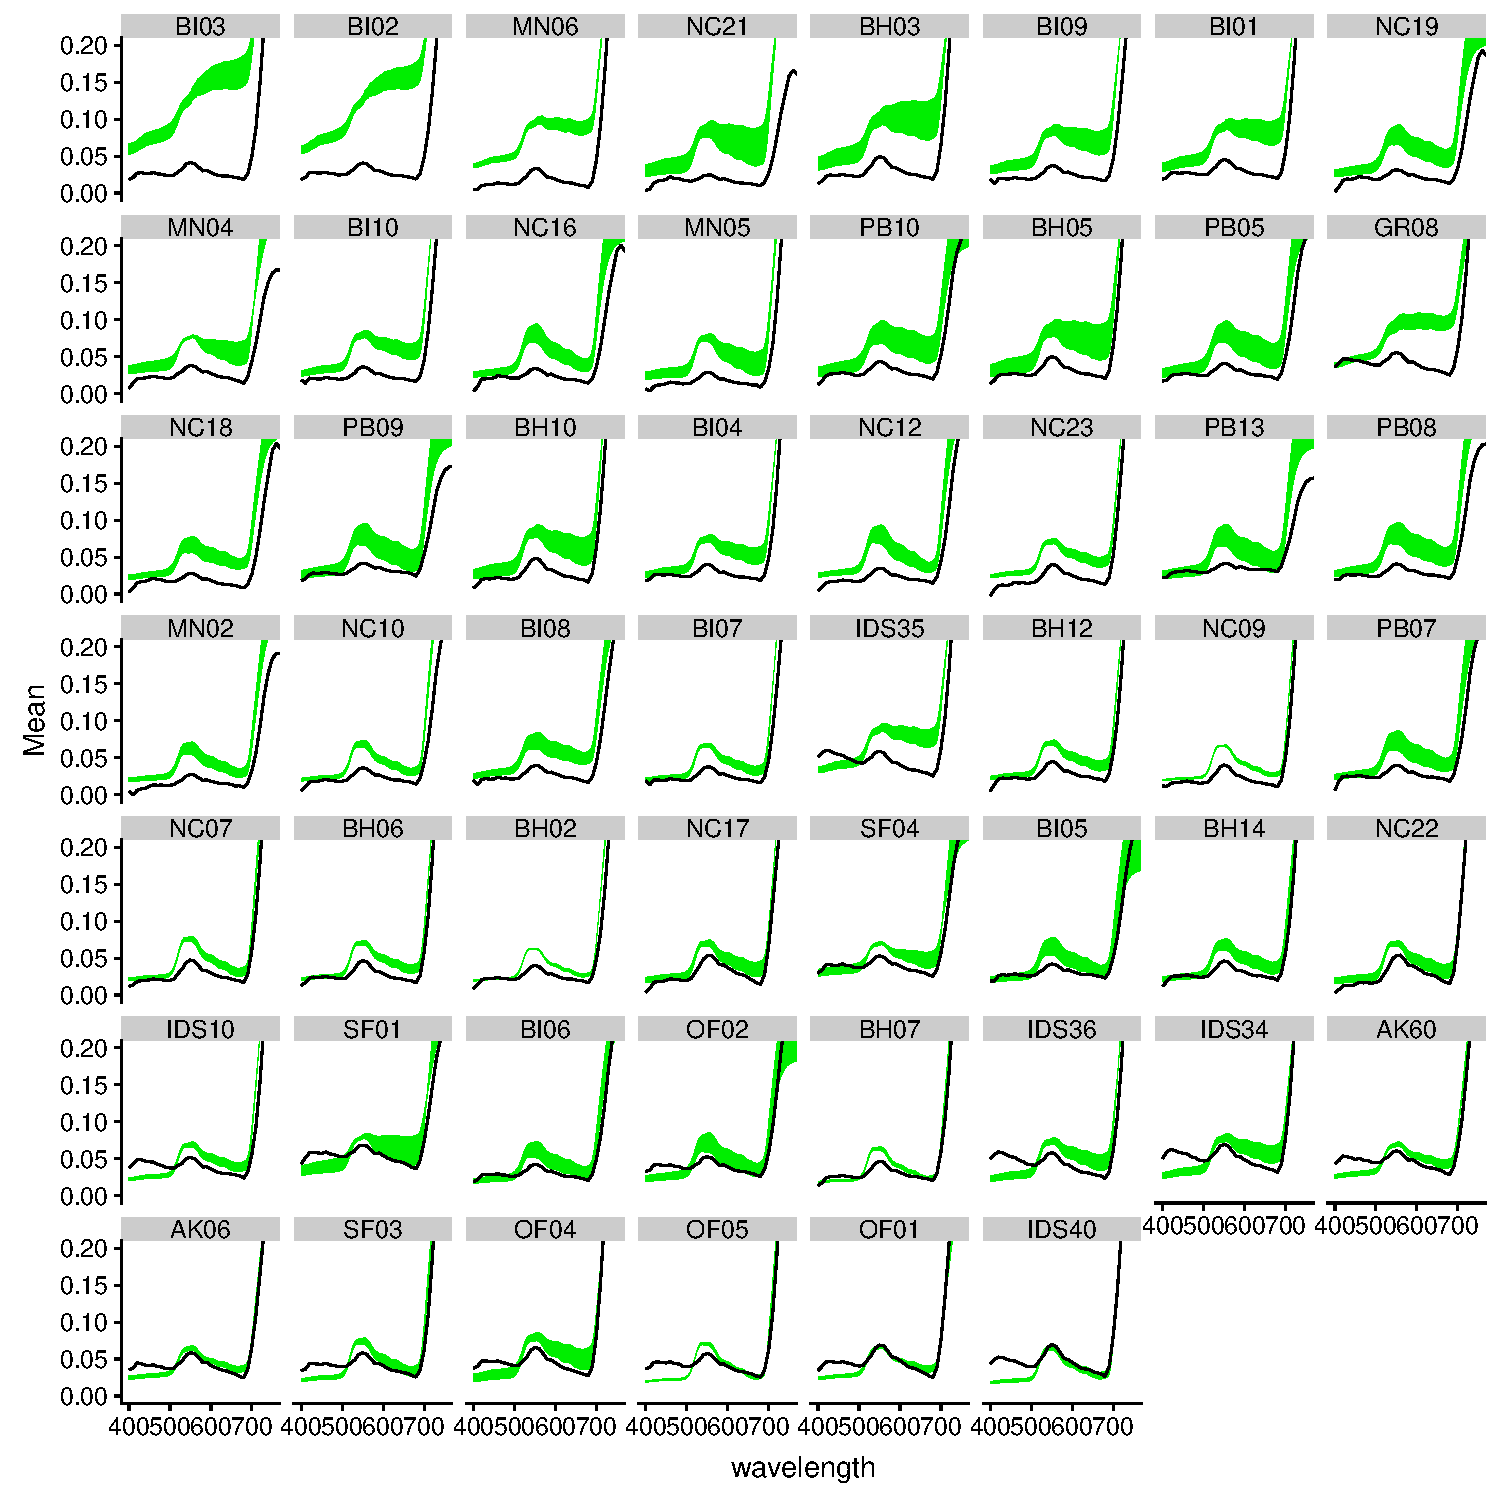
\includegraphics[width=\textwidth]{4_edr/figures/explore_spectra/errors_byvis_vis.pdf}
  \caption{%
    Same as Figure \ref{fig:spec_error_all}, but zoomed into the visible ($<$750 nm) spectral region.
  }\label{fig:spec_error_vis}
  % TODO: Same as above
\end{figure}

\begin{figure}
  \centering
  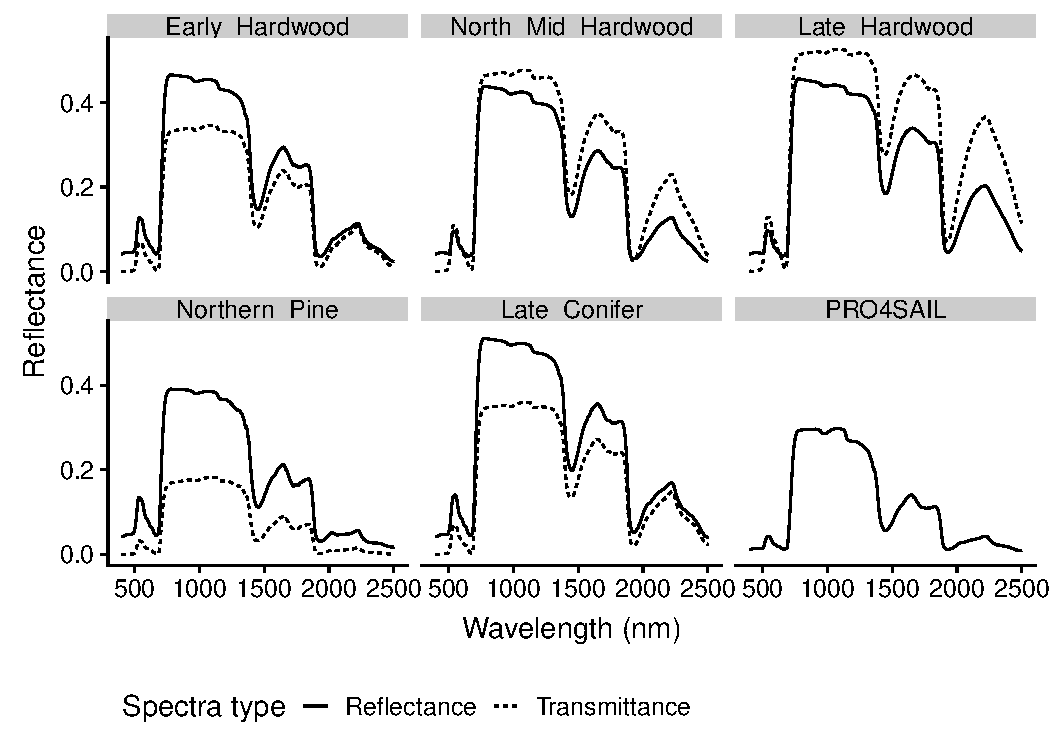
\includegraphics[width=\textwidth]{4_edr/figures/explore_spectra/pft_prospect_sim.pdf}
  \caption{%
    First five panels are PROSPECT simulations of leaf reflectance and transmittance for the plant functional types used in this analysis, based on parameters at their posterior means.
    The final panel is a simulation using the PRO4SAIL~\cite{verhoef_1984_sail} canopy radiative transfer model, parameterized with default structural parameters and leaf parameters averaged across the posterior means of the five plant functional types.
    % TODO: Add SAIL simulation
  }\label{fig:prospect_posterior}
\end{figure}

The ability of EDR to reproduce observed spectra at every site was strongly site-dependent (Figure~\ref{fig:spec_error_all}).
At a majority of the sites, EDR systematically over-predicted reflectance in the visible range (Figure~\ref{fig:spec_error_vis}), while errors in the near-infrared region were more variable.
Given that leaf transmittance is consistently lower than leaf reflectance in the visible range (Figure~\ref{fig:prospect_posterior}), this suggests that the balance of leaf reflectance and transmittance effects on canopy albedo in EDR are unbalanced in favor of the former.

%\begin{figure} \centering
  %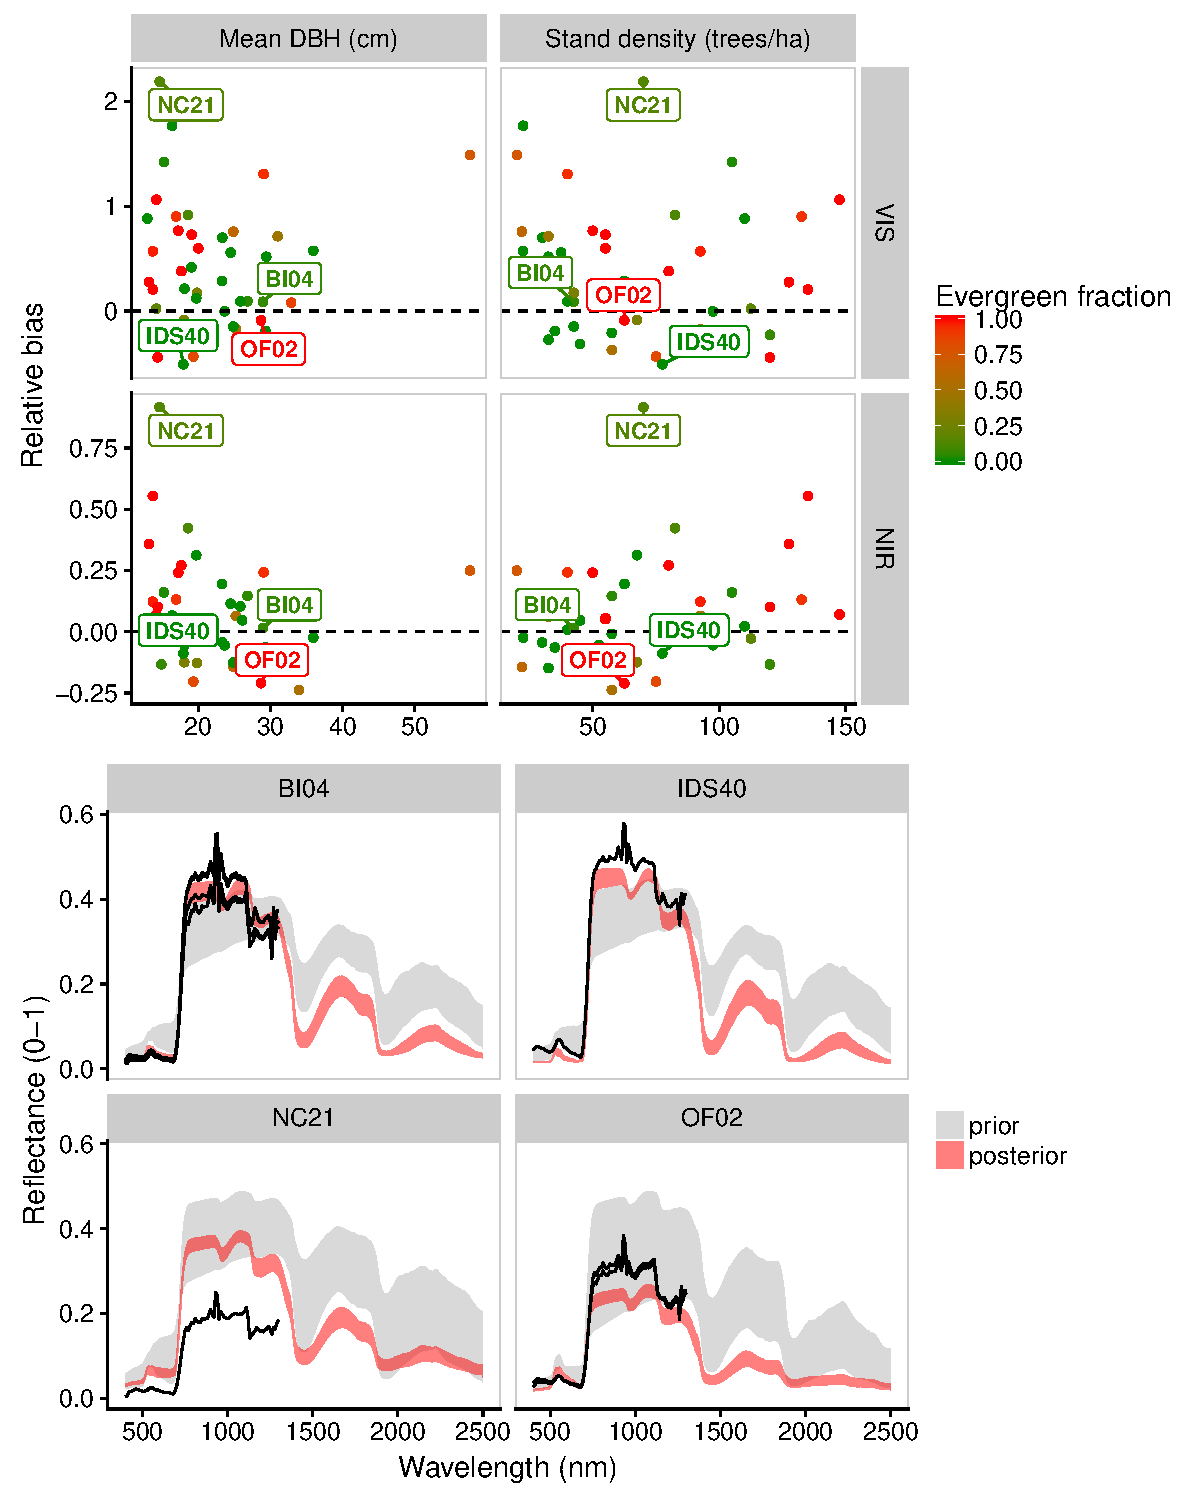
\includegraphics[width=\textwidth]{4_edr/figures/spec_validation.pdf}
  %\caption{\
    %(\textit{Top}) Relative bias of the posterior mean spectra at each site, aggregated across the visible (VIS, 400--750 nm) and near-infrared (NIR, 750--1300 nm) spectral range
    %as a function of site mean diameter at breast height and stand density.
    %(\textit{Bottom}) Prior and posterior predictive intervals and AVIRIS observations for four sites representative of different kinds of error.
  %}\label{fig:bias}
%\end{figure}

%In general, after calibration across a large number of structurally and functionally diverse sites, EDR was able to reproduce observed AVIRIS canopy reflectance reasonably well.  However, performance was strongly site specific.
%At many sites, but most prominently those composed of small trees (DBH < 20, e.g.\ site NC21), EDR frequently overestimated canopy reflectance.
%That being said, least-squares linear regressions of relative spectral bias as a function of site mean DBH or stand density were not statistically significant ($p > 0.1$).
%EDR was generally more likely to overestimate canopy reflectance for conifer trees than broadleaved trees.

\begin{figure}
  \centering
  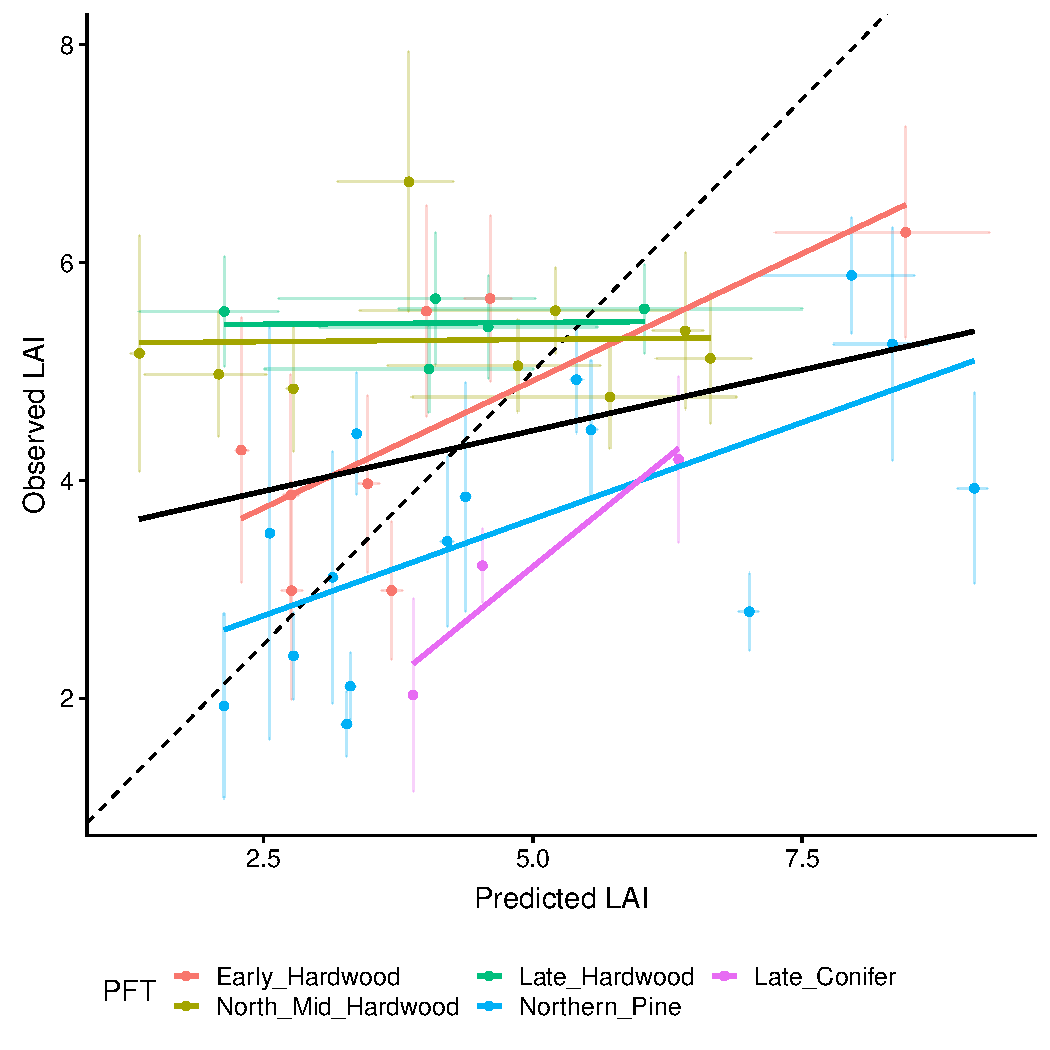
\includegraphics[width=\textwidth]{4_edr/figures/explore_spectra/lai_scatter.pdf}
  \caption{\
    Predictions of leaf area index by EDR, compared to observed values.
    Colors indicate the plant functional type of the tallest cohort at each site.
    % TODO: Add by-PFT regression line
  }\label{fig:lai_validation}
\end{figure}

\begin{figure}
  \centering
  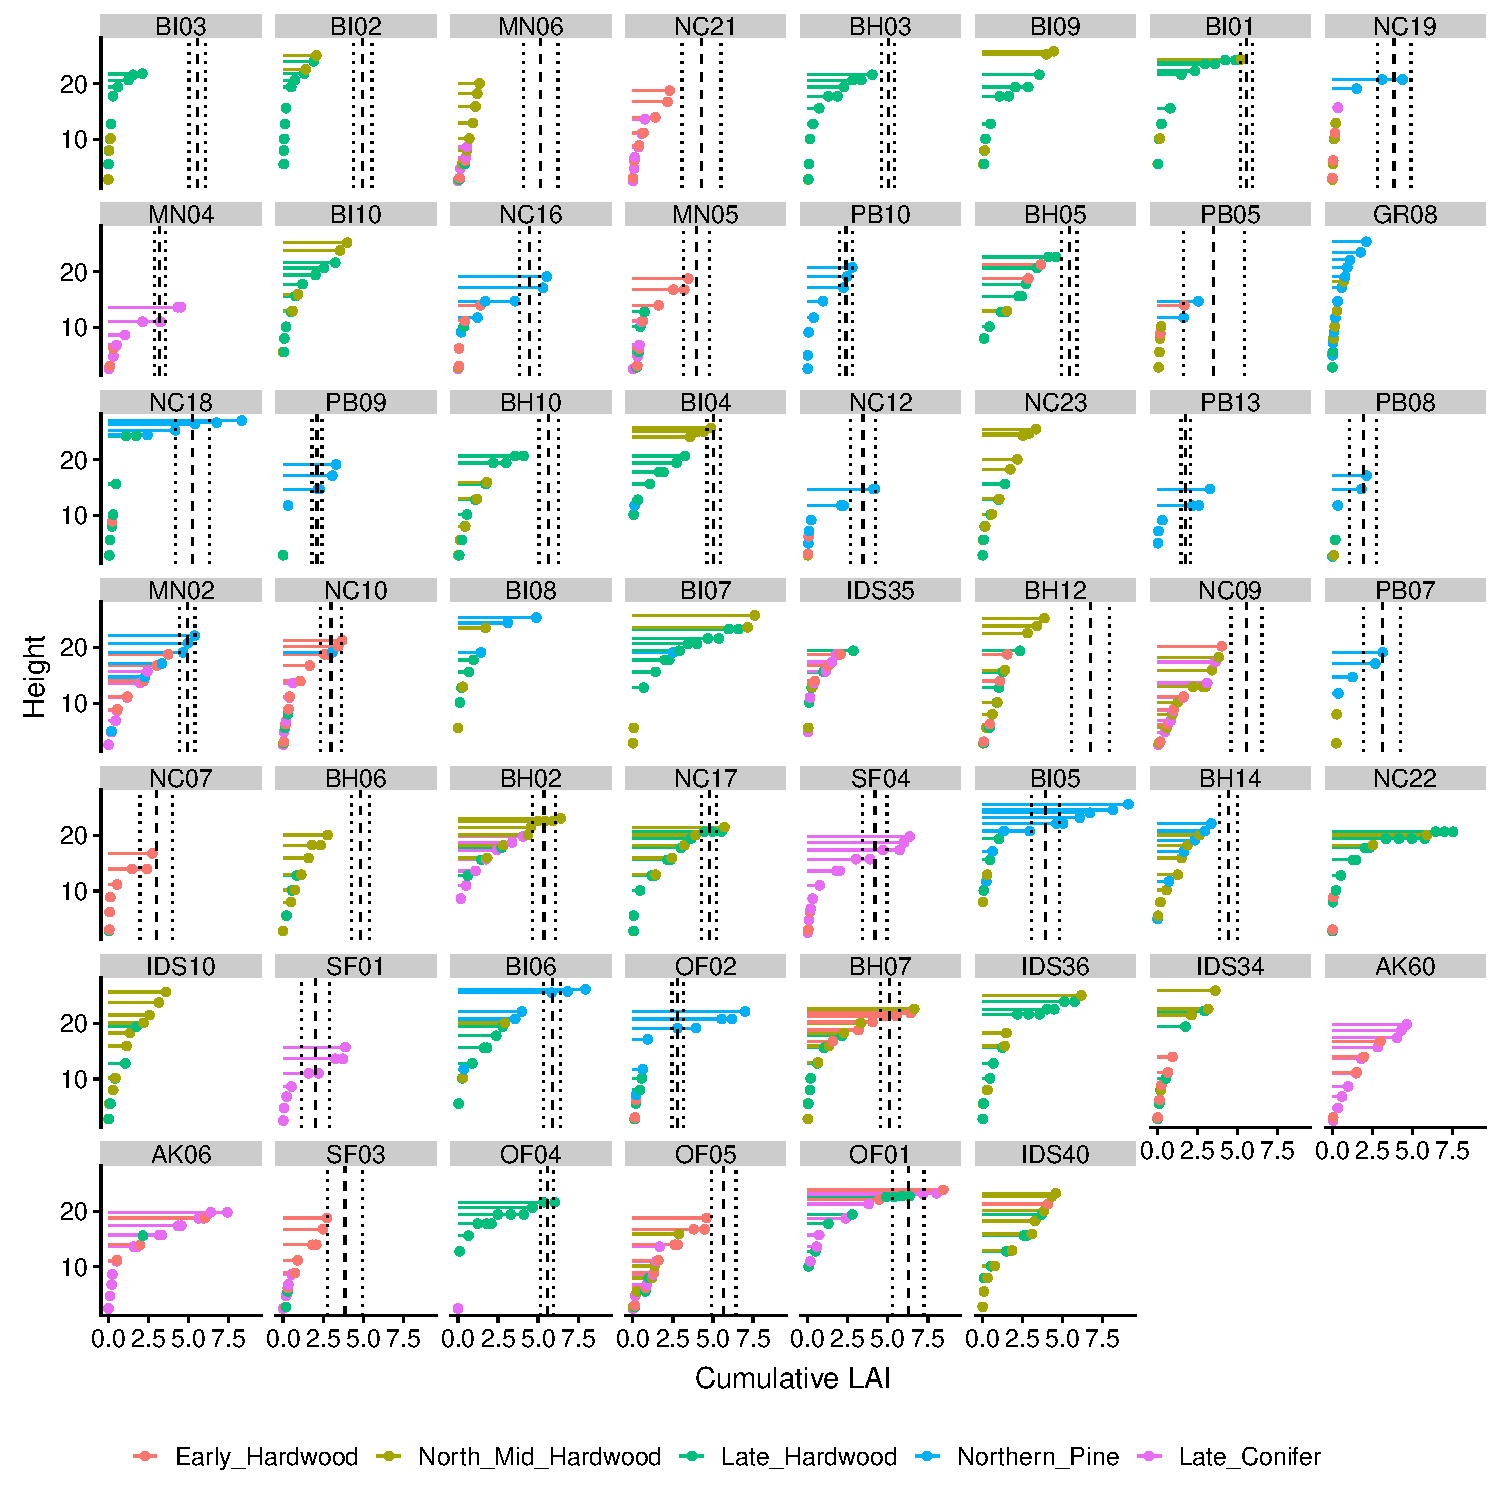
\includegraphics[width=\textwidth]{4_edr/figures/explore_spectra/ed_cumlai_plot.pdf}
  \caption{%
    Vertical profile of cumulative leaf area index and composition at each site in this analysis.
    Vertical black lines indicate the mean $\pm$ 1 standard deviation of the observed leaf area index.
    Sites are arranged in order of decreasing mean error in the visible range, as in Figures~\ref{fig:spec_error_all} and~\ref{fig:spec_error_vis}.
  }\label{fig:lai_profile}
\end{figure}

The ability of EDR to reproduce observed leaf area index was also strongly site-dependent, with some of the accuracy explained by the functional type of the tallest cohort (Figures~\ref{fig:lai_validation} and~\ref{fig:lai_profile}).
In general, EDR tended to over-predict leaf area index for conifer-dominated stands and under-predict for hardwood-dominated stands.
For mid- and late-hardwood-dominated stands in particular, EDR predicted substantial variability in leaf area index that was not present in the observations.

%\begin{figure}
  %\centering
  %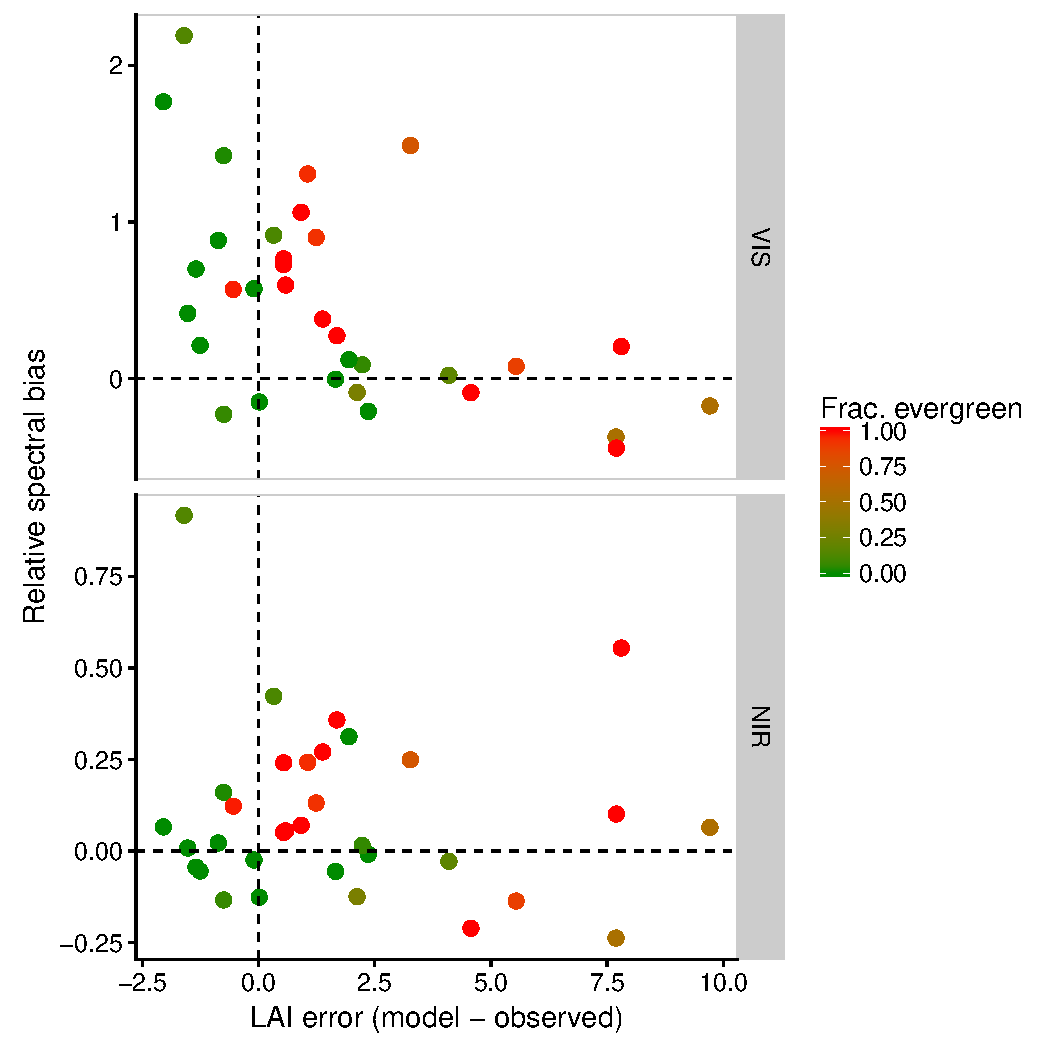
\includegraphics[width=\textwidth]{figures/spec_lai.pdf}
  %\caption{\
    %Relationship between errors in EDR predictions of leaf area index and spectra.
  %}\label{fig:spec_lai}
%\end{figure}

%There was a significant negative relationship between EDR LAI errors and spectral errors in the visible range;
%in other words, EDR tended to overestimate either LAI or canopy reflectance.

%\subsection{Forward simulation}
%\begin{figure}
  %\centering
  %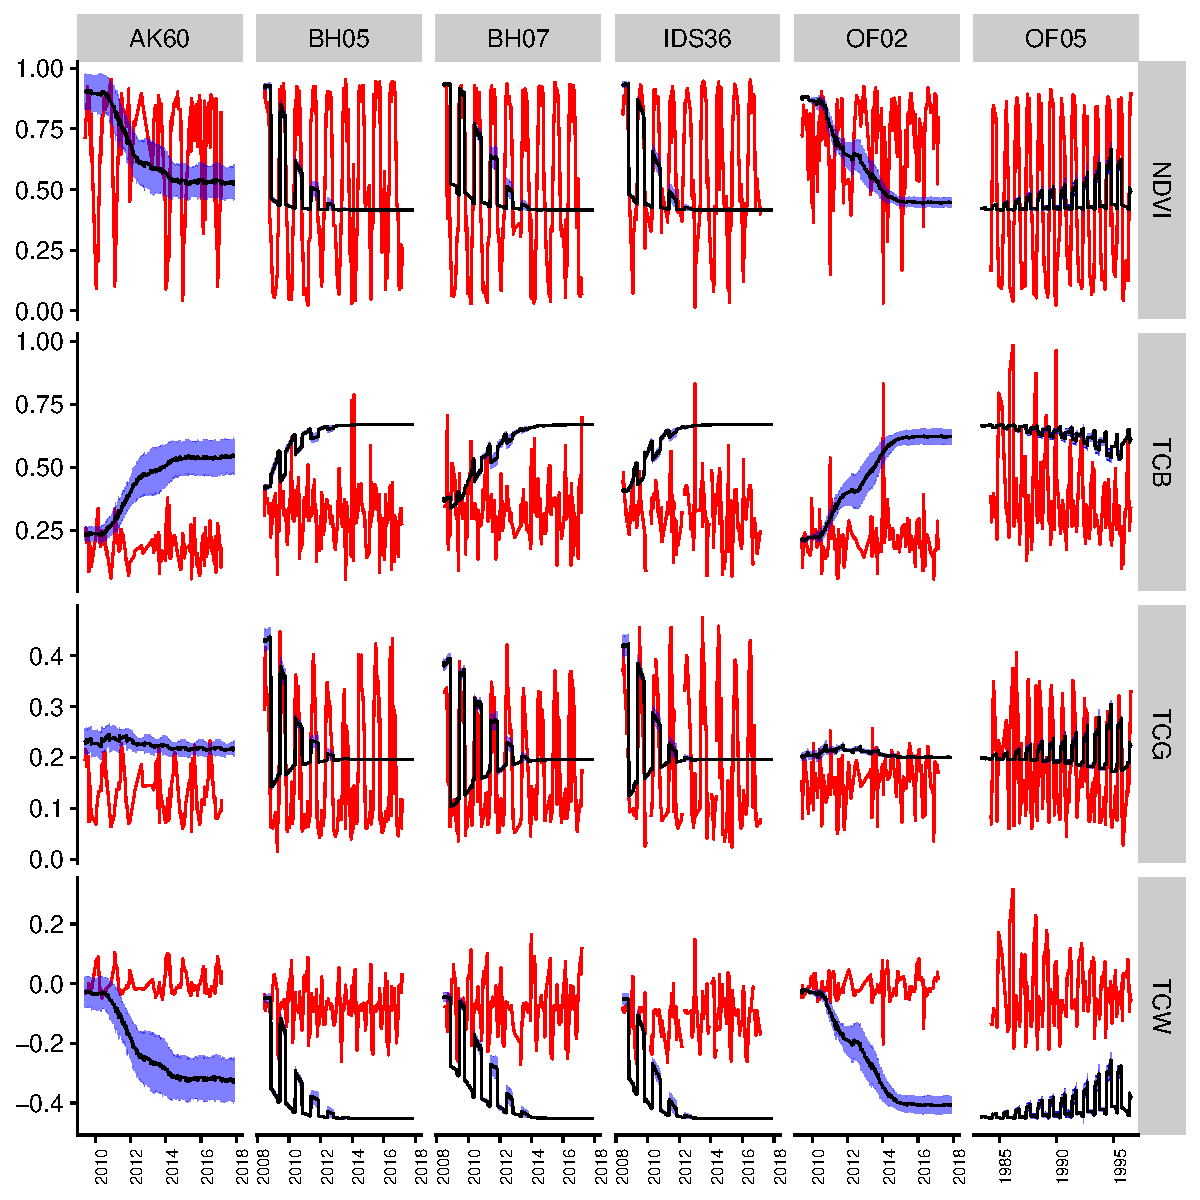
\includegraphics[width=\textwidth]{figures/landsat_ts.pdf}
  %\caption{\
    %Comparison of EDR-simulated (black, blue ribbon) and observed (red) time series of Landsat NDVI and tasseled cap brightness (TCB), greenness (TCG), and wetness (W) for each site.
  %}
%\end{figure}
%(Currently working on this text\ldots).
